\section{Results and Discussion}

The \texttt{dhrystone-dhry} test results drawn in \autoref{fig:dhry-training}
is chosen as the final test for PET as it utilize a wide range of both the
integer parts and memory system of the processors. The Dhrystone benchmark will
provide a scenario where all input weights for PET at least must add up to the correct
overall power drain. There is, of course, a chance that the values are weighted wrongly, but
still matches the sum of the real power drain. We cannot guarantee that 


\begin{figure}[ht]
\centering
\includegraphics[width=\textwidth]{figs/training/dhrystone-dhry.pdf}
\caption{Overlay of PET training results (red) and training data (green).}
\label{fig:dhry-training}
\end{figure}

\subsection{Explanations and Errors}
The estimates given by PET is clearly created from a very high level of abstraction,
and will never have enough information to exactly resemble the power profile of
the realized chip. However, given that the power consuming events are carefully
selected and well weighted, the current results indicate that this method works quite well.

\begin{figure}[ht]
    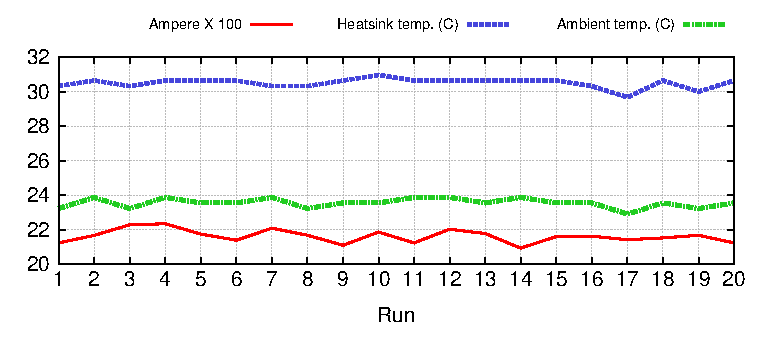
\includegraphics{figs/heat}
    \caption{Variations in measurements.}
    \label{fig:variation}
\end{figure}

In \autoref{fig:variation}, recreated from Fig. 8 in \cite{rundehvatum2013exploring} which uses exactly the
same power measurement setup, it is clear that the measured current drain varies over
time seemingly uncorrelated to both on-chip and ambient temperature. Each data point
in the figure represents the results from a test run of the \texttt{add-add} test with
about one hour between each run. The results ranges from $208~mA$ to $224~mA$ and averages to $216~mA$.
The results can be written as:
\[I_{add} = 216~mA\pm8~mA = 216~mA\pm3.8~\%\]

With a measured error of $\pm3.8~\%$ it is not unreasonable to calculate a $10~\%$ error in
all measurements. This means that the weights found using measurements and a genetic algorithm might
have had a slight discrepancy between each training set, which again makes renders it impossible to get
correct results. It would be possible, that by chance, some genome would fit all training set even though
they contains errors, but the weights would most likely not be equal to the ''correct`` weights.

It is also such that most search algorithms are prone to a phenomenon called
over-fitting \cite{russellnorvig}.  Over-fitting happens because the genetic
algorithms will find any kind of patterns, so if a higher power drain was seen
randomly, but a specific event often happens at the same time as the power
drain, the algorithm would try to blame the event for the drain, even if a human
would exclude it as it not always correlating.

\begin{figure}[ht]
\centering
\includegraphics[width=\textwidth]{figs/training/add-add.pdf}
\caption{Overlay of PET training results (red) and training data (green).}
\label{fig:add-training}
\end{figure}

The \texttt{add-add} test which is displayed in \autoref{fig:add-training} is
especially interesting because is utilized the fast-loop mode of the Cortex-A9.
This means that it would not need to use its L1 cache way near as much as the
simulator thinks, as the simulator does not embed fast-loop. PET would then
predict a higher power drain, as it thinks that the caches are in use. This is
a problem one must be aware of when the simulator and realized hardware does not
completely corresponds to each other. However, the main purpose of PET is to
estimate changes done on simulation level, thus this is not a real problem in the
ordinary usage scenarios.

It is also clear from \autoref{tbl:gem5runtimeaccuracy} that the CPU model used
in gem5 is not exactly equal to the Cortex-A9 core used in the Samsung Exynos
4412 Prime SoC, thus each graph in both training and results are stretched to
match each other. This is certainly a source of error, but from
\texttt{trend-trend} in \autoref{fig:trend-training} and \texttt{trend-submul}
in \autoref{fig:submul-training} it is reasonable to believe that the scaling
works, as the change in program flow is shown not far from each other in the
predicted graph and real measurement graph.
